\begin{figure}[p]
\centering
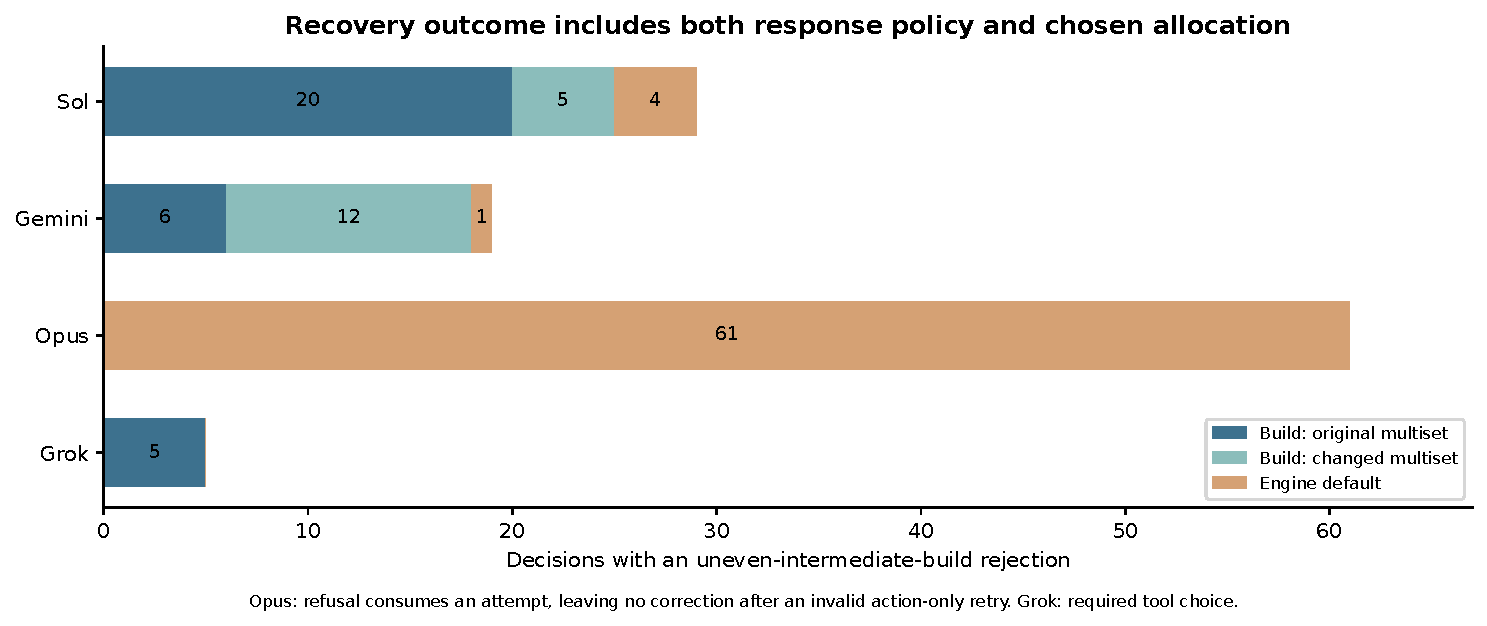
\includegraphics[width=\linewidth,height=4.4in,keepaspectratio]{f07_build_recovery.pdf}
\caption[A legal build after retry need not preserve the proposed allocation]{Population: decisions with an uneven-intermediate-building rejection, not all build opportunities. A successful recovery means some legal construction was applied within the same decision. It preserves the original purchase multiset in 20/25 Sol, 6/18 Gemini and 5/5 Grok recoveries; the others change it. All 61 Opus defaulted plans can execute after interleaving identical purchases, but its refusal/recovery condition leaves no corrective attempt after the invalid action-only retry. One chain has the reversed order of invalid attempt then refusal. These are configured-system mechanics; the chart neither imputes repaired outcomes nor proves a causal loss of wins. Eventual same-turn target attainment is separate from within-decision preservation. Source: Sol's exact-plan and full-event replay audit, independently challenged by all peers. Underlying data: Table~\ref{tab:t07_build_recovery}.}
\label{fig:f07_build_recovery}
\end{figure}
